\section{people}

If interdisciplinary research and teaching are to thrive, in addition to a positive hiring policy there needs to be good career development for those that undertake it.
 In general, it is possible to affirm that the situation,
even if significantly different from case to case, reveals a
significant level of immaturity that will have to be overcome in the
near future if interdisciplinary research and teaching are to thrive. The good news is that some universities, even if in
a non-completely structured way, are investing significant effort to
increase the presence of interdisciplinary faculty among research and
teaching staff. More time is certainly needed to assess the
effects of these investments and to see a change in the most
conservative countries in Europe. The 
following subsections discuss the answers obtained for each specific
question.

\subsection{Interdisciplinary hiring}\label{sec:hiring}

\begin{figure}[h]
\centering
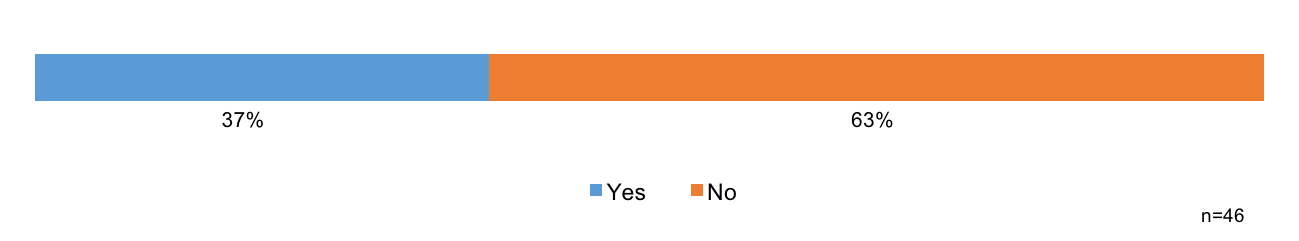
\includegraphics[width = \linewidth]{charts/3a.png}
\caption{Does your university explicitly hire academics
  who focus on interdisciplinary research?}
\label{sect3:hirings}
\end{figure}

63\% of the respondents have affirmed that their university does not
explicitly hire interdisciplinary researchers (see Figure~\ref{sect3:hirings}). In Italy this is 
due to the organization of research areas in distinct \emph{scientific
  sectors}, which are mostly related to a single discipline and cannot be easily revised to follow the advances of
research and technology. Spain appears to show similar problems.

Among the 37\% of positive respondents, some identify bioinformatics
as one of the areas where multidisciplinary researchers are hired. 
Other identified areas concern human-machine interaction, medical
informatics, AI/data science, and media informatics/game design.

\subsection{Affiliation of interdisciplinary faculties}
\begin{figure}[h]
\centering
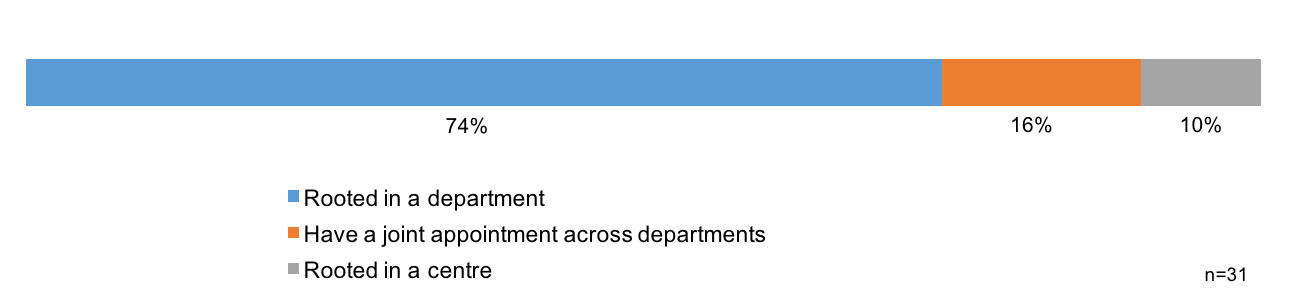
\includegraphics[width = \linewidth]{charts/3b.png}
\caption{Are faculty rooted in a department, have a joint appointment across departments, or rooted in a centre?}
\label{sect3:affiliation}
\end{figure}

In 74\% of the cases, multidisciplinary researchers are rooted within
a department (see Figure~\ref{sect3:affiliation}). 
According to the comments associated to this question,
this seems to be due to the need to assign every faculty to a specific
department. The respondents, however, note that such researchers spend
also part of their time in a multidisciplinary centre or in another
department. 

\subsection{Assessment of interdisciplinary faculties}


\begin{figure}[h]
\centering
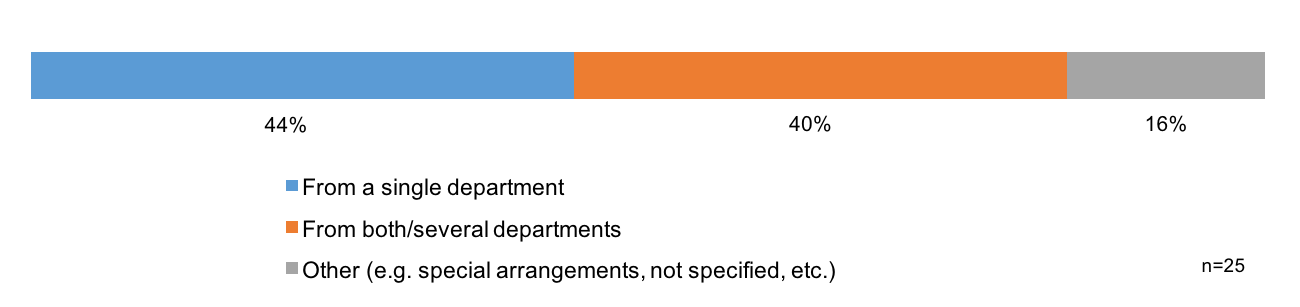
\includegraphics[width = \linewidth]{charts/3c.png}
\caption{How is their quality judged for both appointment and for promotion?}
\label{sect3:assessment}
\end{figure}

As shown in Figure~\ref{sect3:assessment}, there is an equal distribution between universities
where the appointment/promotion assessment is performed at the
department level and universities where this happens across
departments. Analysing the specific comments by the respondents, it is
difficult to find common patterns as the mechanisms for appointing and
promoting faculties appear to vary significantly from country to
country. 

\subsection{Planned initiatives concerning multidisciplinary hirings}

\begin{figure}[h]
\centering
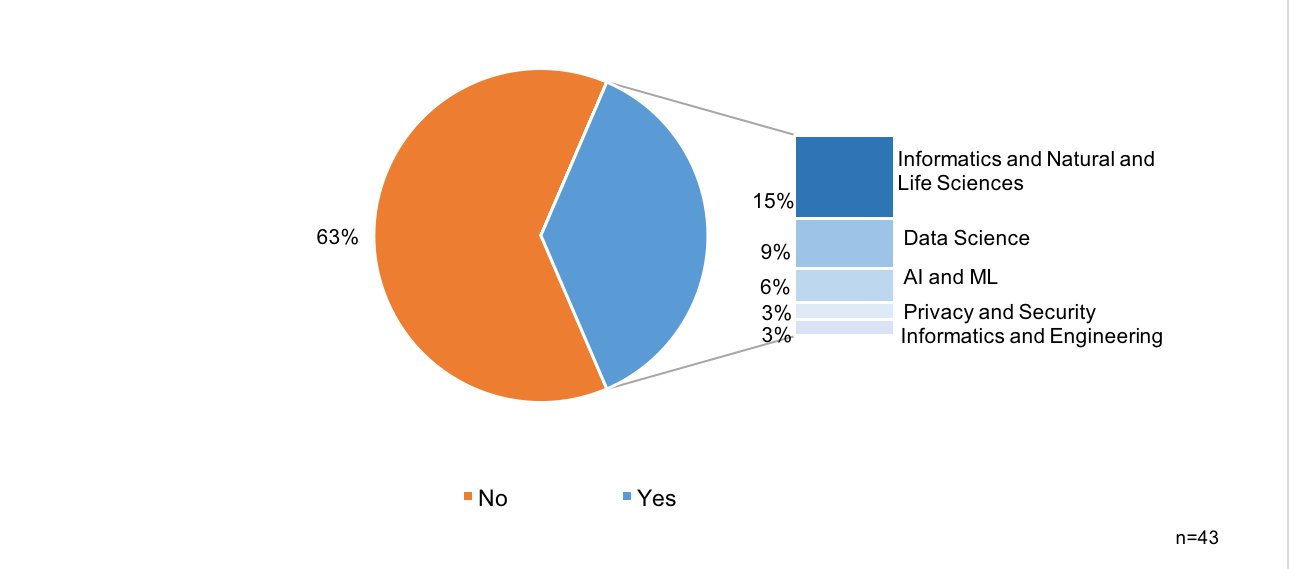
\includegraphics[width = \linewidth]{charts/3d.png}
\caption{Are there any initiatives planned to hire in interdisciplinary areas?}
\label{sect3:planned}
\end{figure}

As shown in Figure~\ref{sect3:planned}, the answer to this question correlates to the ones
discussed in Section~\ref{sec:hiring}. Also in this case, 63\% of
respondents do not see any plan to hire multidisciplinary researchers
while among those who see these plans in place natural life and
science and, in particular, bioinformatics, appear to be the most
targeted field. 

\subsection{Final thoughts}

The answers to these questions show that the situation is still quite
immature. In the cases where universities are largely autonomous from
national agencies, hiring interdisciplinary researchers is
encouraged when there is some funding, often by third parties, dedicated to
this. Even in this case, respondents highlight the difficulty of comparing
researchers with different background and skills and the current
lack of complete understanding of how to judge interdisciplinary research, given the limited
number of multidisciplinary researchers that are currently in the
system. 

Respondents from countries where the hiring system is strongly
regulated by some national agency, highlight the difficulty to
introduce some flexibility and to define long-term plans
which include multidisciplinarity as an important aspect. 
